\begin{figure}
	\centering
	\begin{subfigure}{0.8\linewidth}
		\centering
		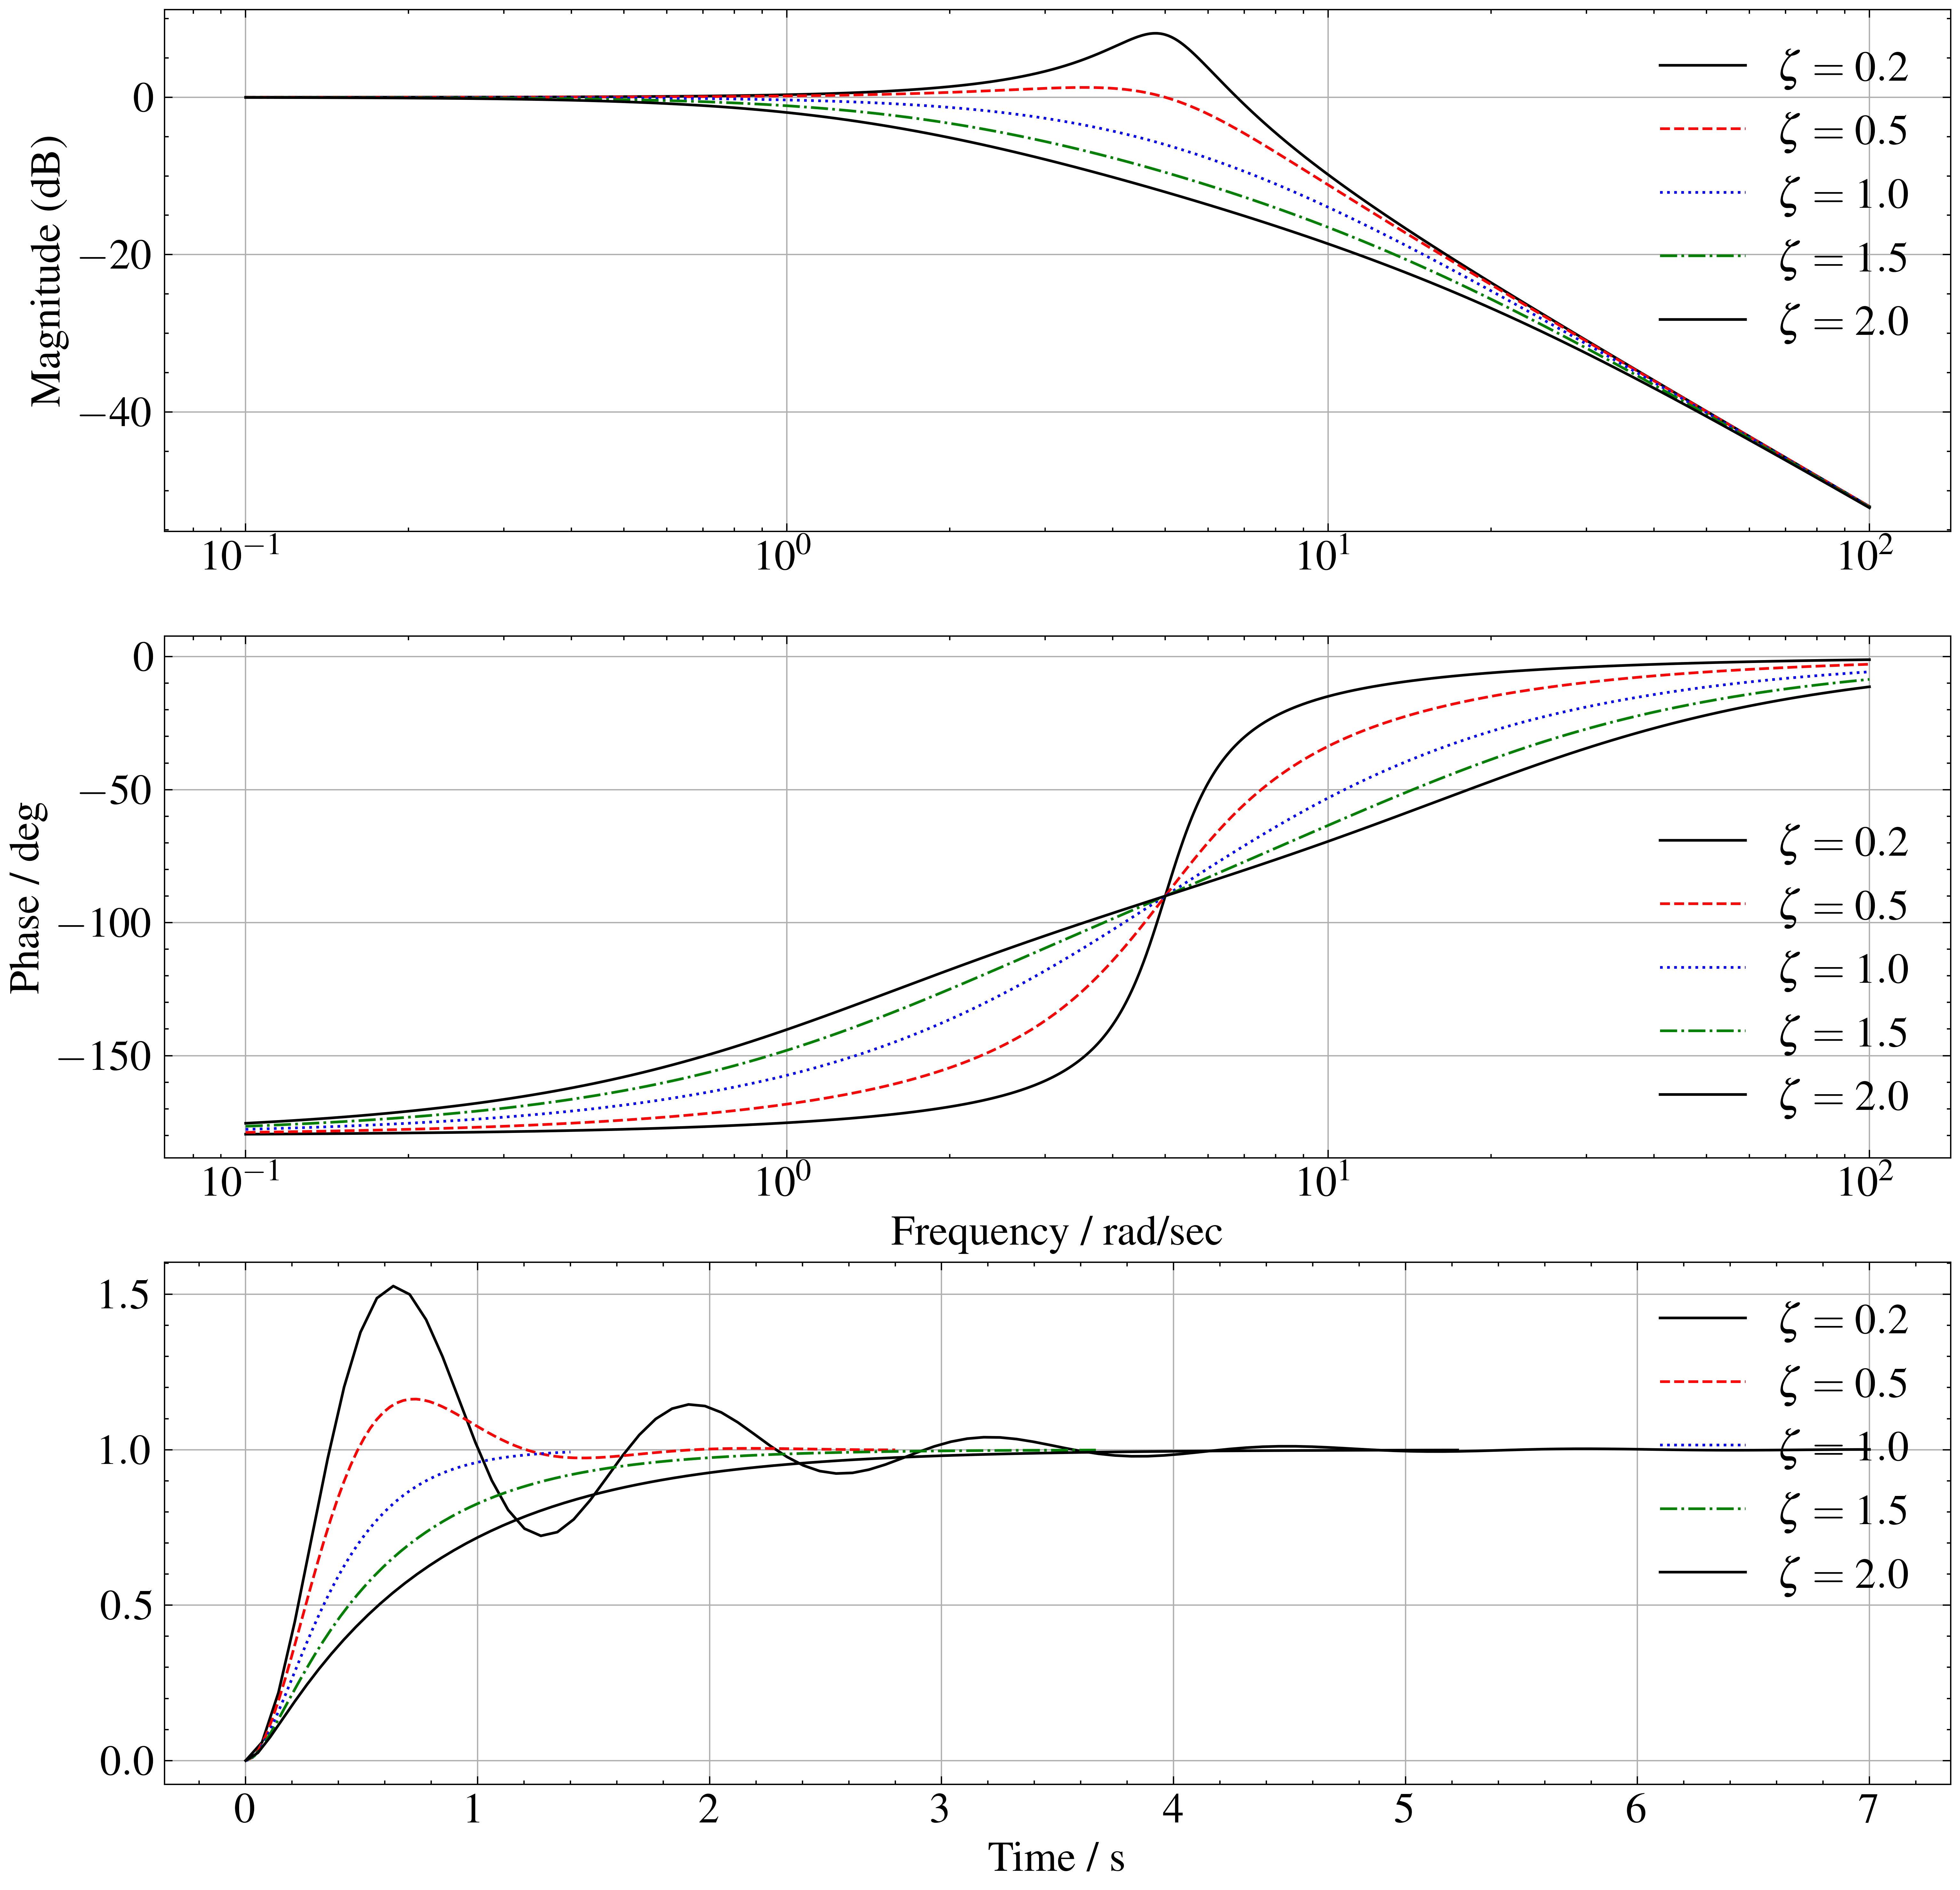
\includegraphics[width=0.8\linewidth]{src/figures/bode-phase-step-ideal-group-omega/bode-phase-step-ideal-group-omega-5.png}
		\subcaption{$\omega = 5$}\label{fig:bode-phase-step-ideal-group-omega-5}
	\end{subfigure}
	\begin{subfigure}{0.8\linewidth}
		\centering
		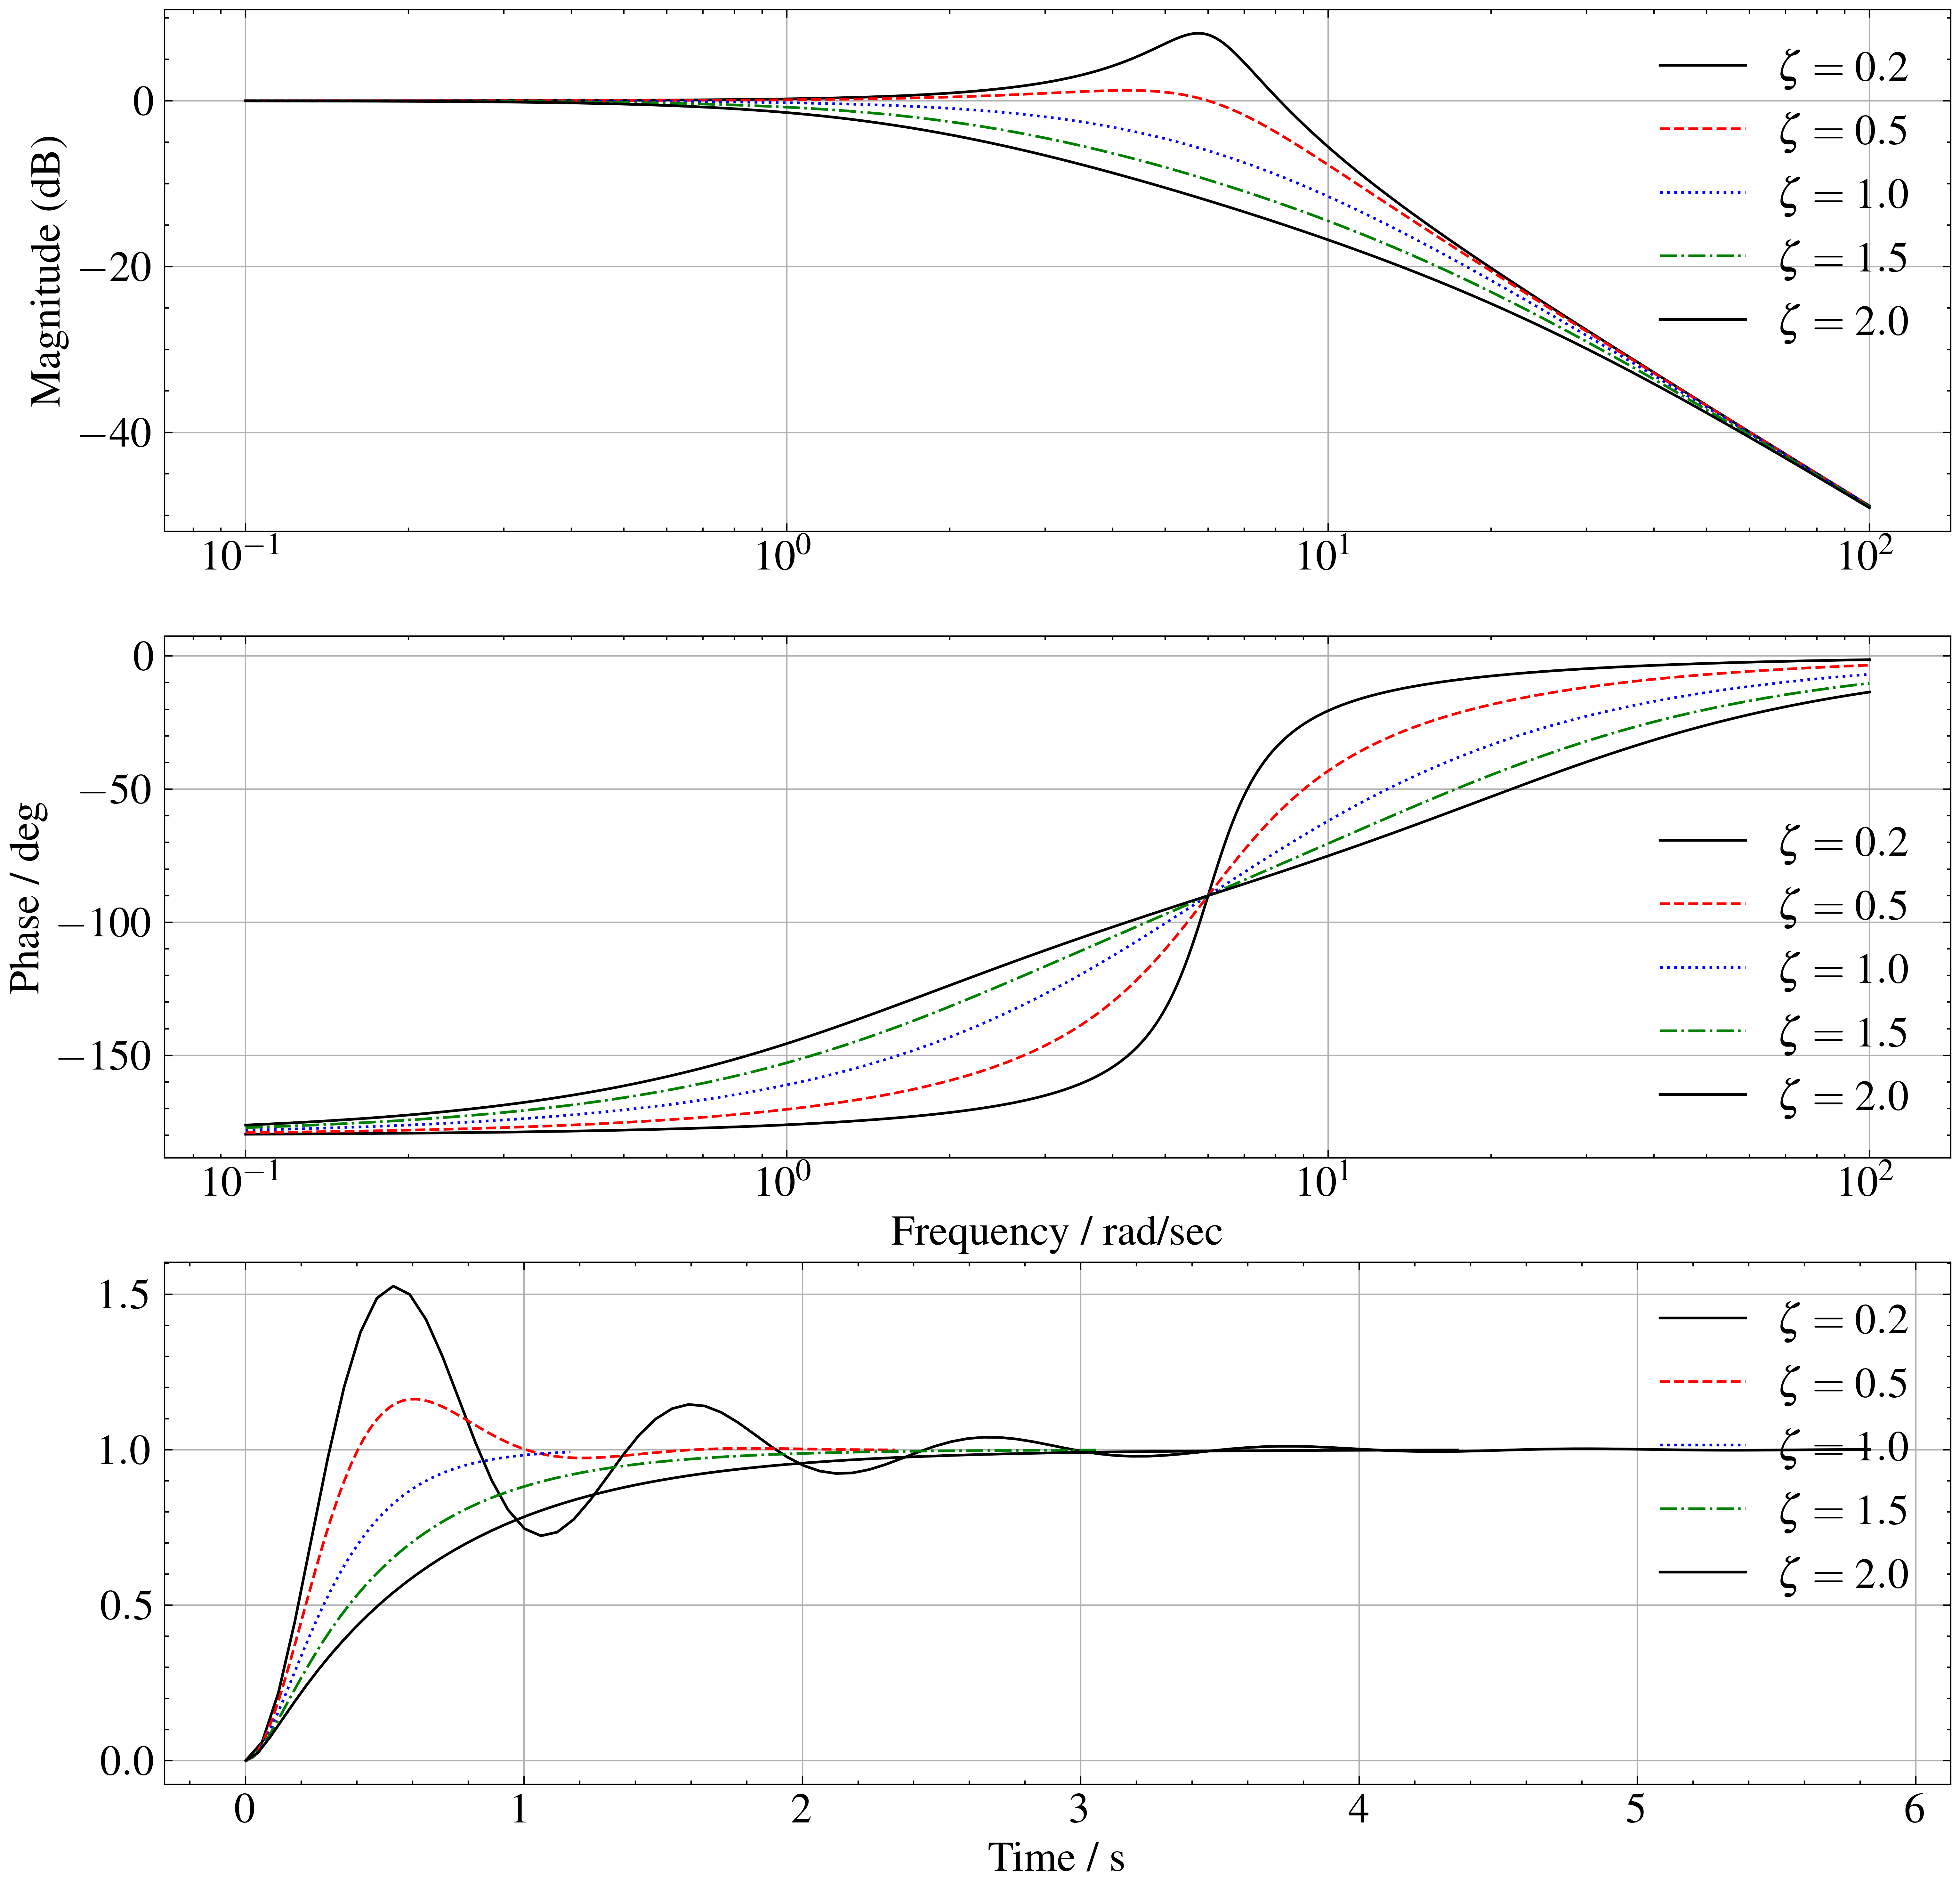
\includegraphics[width=0.8\linewidth]{src/figures/bode-phase-step-ideal-group-omega/bode-phase-step-ideal-group-omega-6.png}
		\subcaption{$\omega = 6$}\label{fig:bode-phase-step-ideal-group-omega-6}
	\end{subfigure}
	\caption{ある$\omega$に対して、$\zeta$を変化させたときのボード線図とステップ応答}\label{fig:bode-phase-step-ideal-group-omega}
\end{figure}


\begin{figure}
	\centering
	\addtocontents{figure}{-1}
	\begin{subfigure}{0.8\linewidth}
		\setcounter{subfigure}{2}
		\centering
		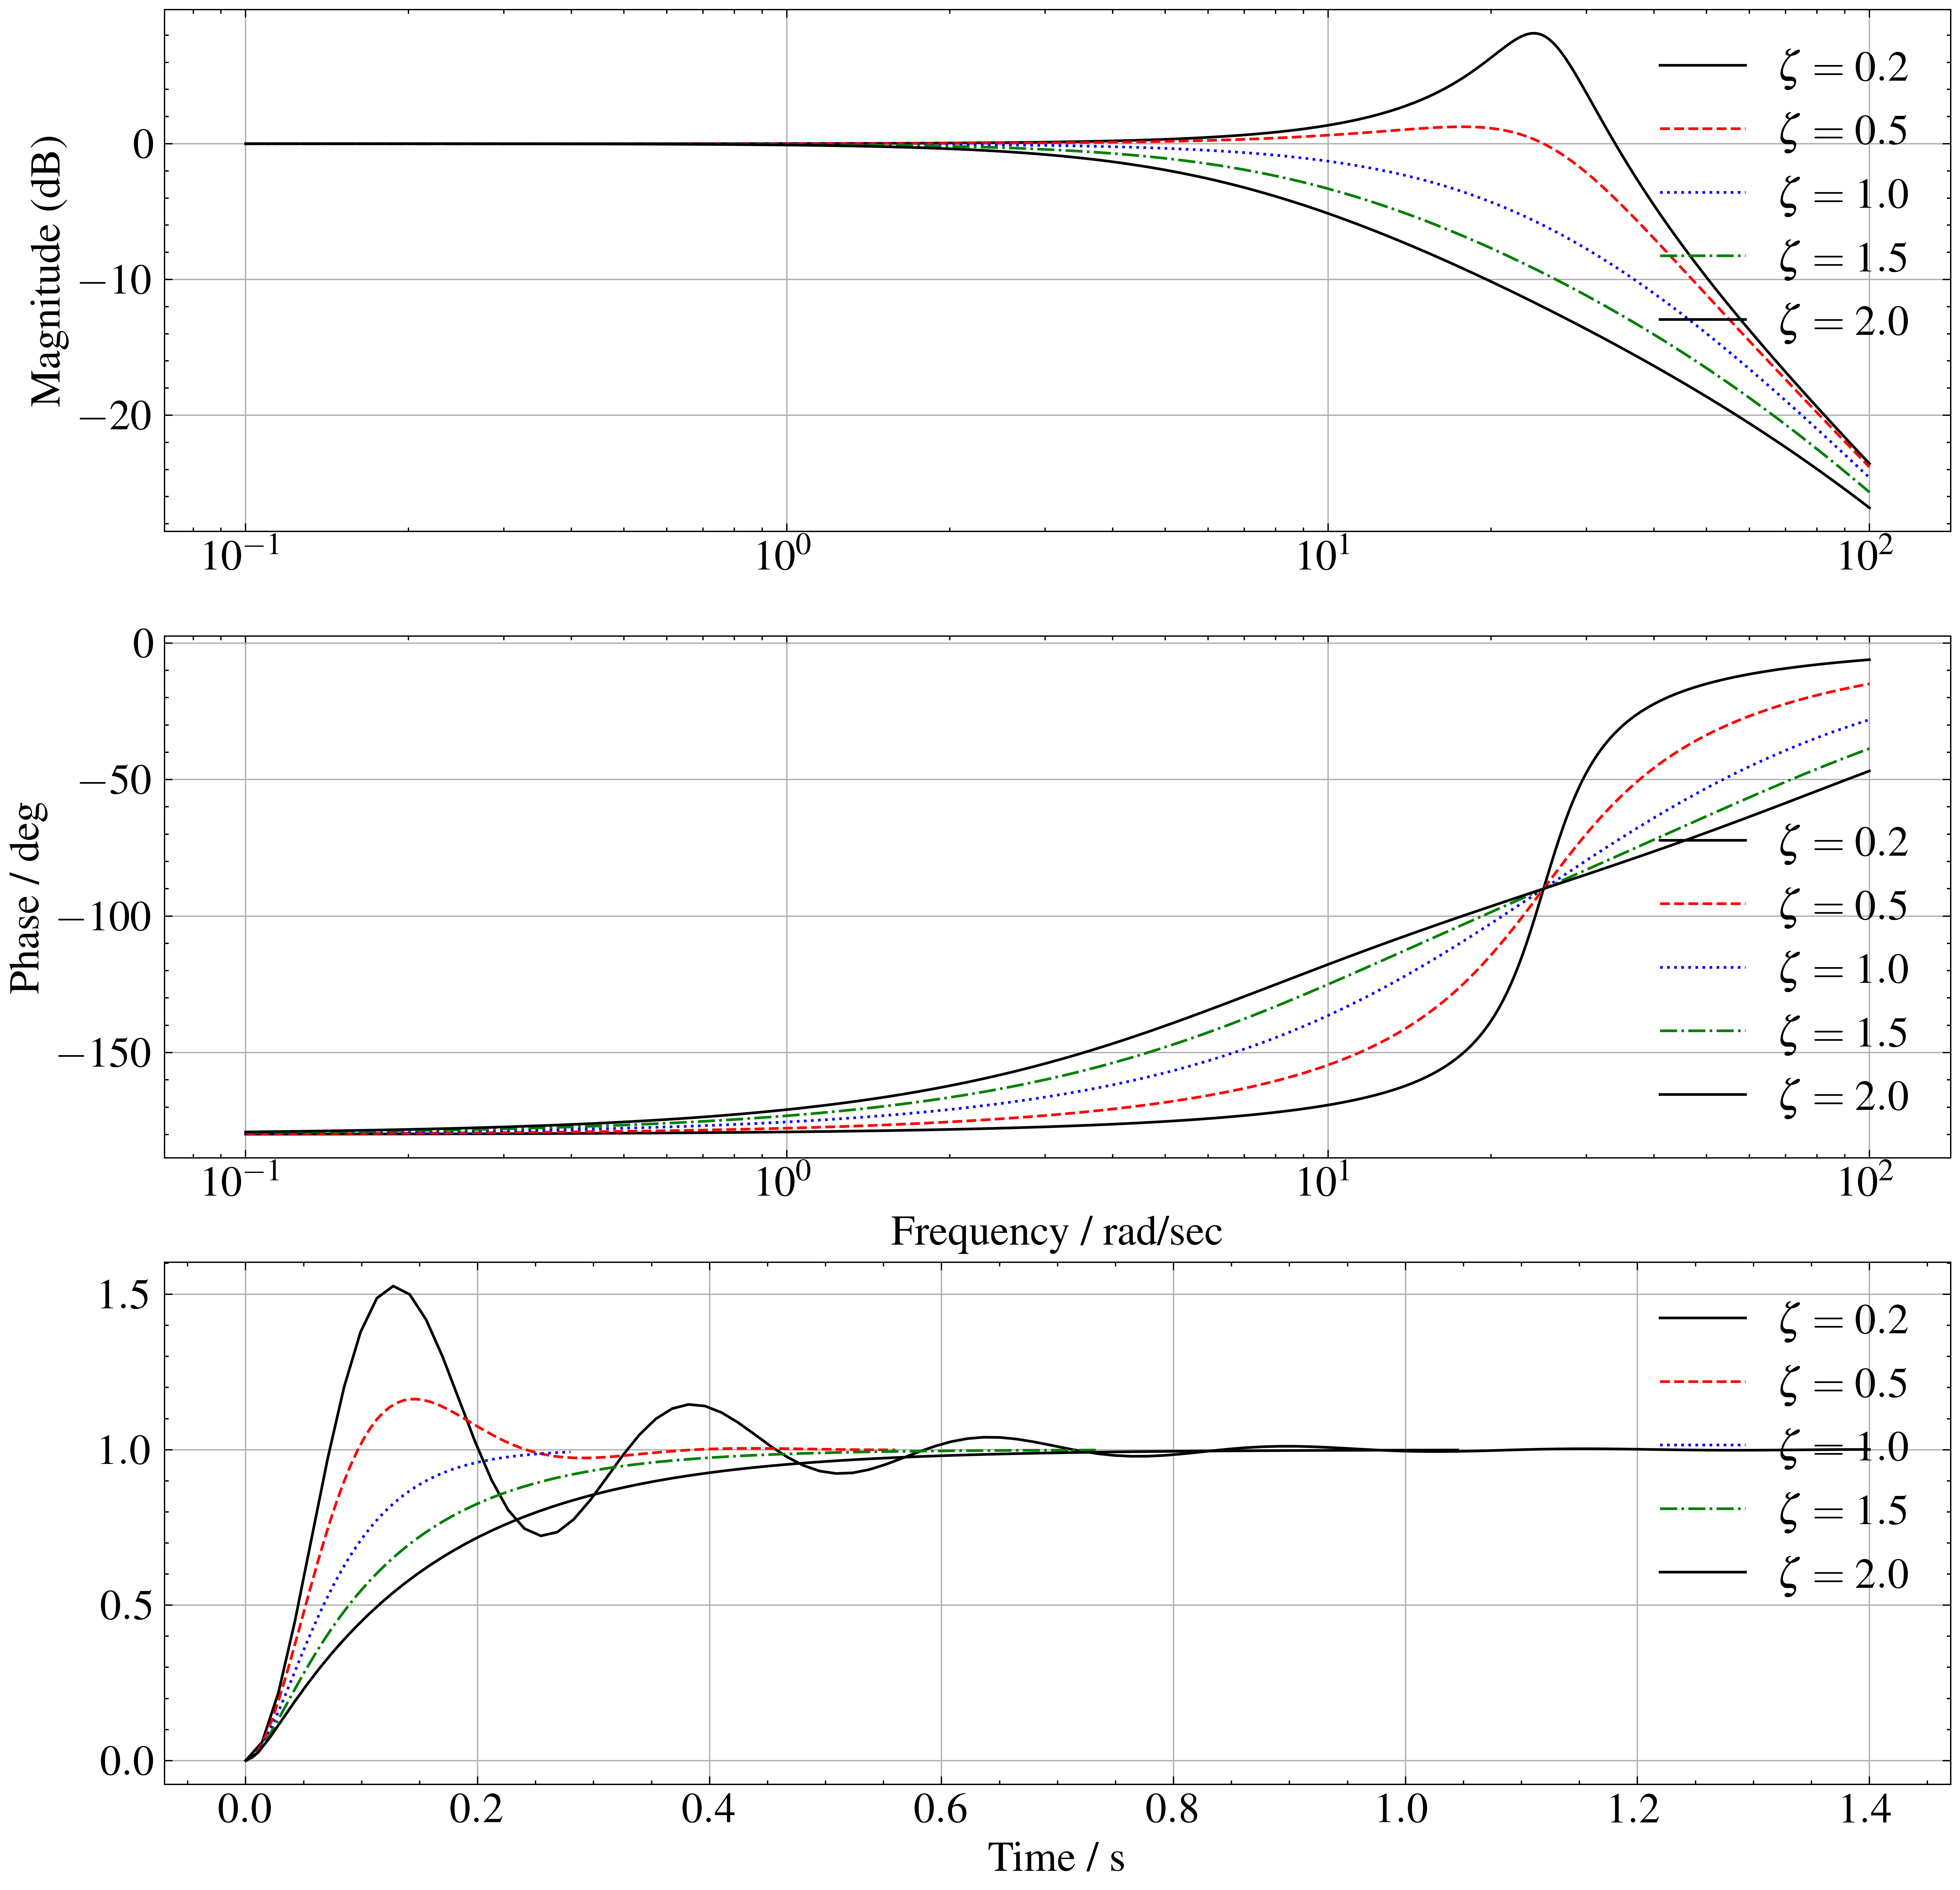
\includegraphics[width=0.8\linewidth]{src/figures/bode-phase-step-ideal-group-omega/bode-phase-step-ideal-group-omega-25.png}
		\subcaption{$\omega = 25$}\label{fig:bode-phase-step-ideal-group-omega-25}
	\end{subfigure}
	\caption{ある$\omega$に対して、$\zeta$を変化させたときのボード線図とステップ応答(続き)}
\end{figure}
